%%%%%%%% ICML 2026 EXAMPLE LATEX SUBMISSION FILE %%%%%%%%%%%%%%%%%

\documentclass{article}

% Recommended, but optional, packages for figures and better typesetting:
\usepackage{microtype}
\usepackage{graphicx}
\usepackage{caption}
\usepackage{booktabs} % for professional tables
\usepackage{listings}
\usepackage{xcolor} % optional, for syntax highlighting
\usepackage{float} % for H placement
\usepackage{tabularx}
\usepackage{tikz}
\usetikzlibrary{arrows.meta, positioning, decorations.pathreplacing, shadows}
\usetikzlibrary{matrix, fit, backgrounds}
\usepackage{placeins}
\usepackage{algorithm}
\usepackage{algorithmic}
\usepackage{pgfplots}
\pgfplotsset{compat=1.18}
\usepackage{subcaption} % For subfigures
\usepackage{epstopdf}   % EPS support in pdflatex


\usepackage{tcolorbox}   % for boxed listings
\tcbset{
    mypythonbox/.style={
        listing engine=listings,
        listing only,
        breakable,
        enhanced,
        colback=gray!5,
        colframe=black,
        boxrule=0.5pt,
        arc=2mm,
        outer arc=2mm,
        left=2mm,
        right=2mm,
        top=1mm,
        bottom=1mm,
        title=#1,
    }
}

% Optional: configure listings for Python
\lstset{
    language=Python,
    basicstyle=\ttfamily\small,
    keywordstyle=\color{blue},
    stringstyle=\color{red!70!black},
    commentstyle=\color{green!50!black},
    numbers=left,
    numberstyle=\tiny,
    stepnumber=1,
    numbersep=5pt,
    breaklines=true,
    showstringspaces=false
}


% hyperref makes hyperlinks in the resulting PDF.
% If your build breaks (sometimes temporarily if a hyperlink spans a page)
% please comment out the following usepackage line and replace
% \usepackage{icml2026} with \usepackage[nohyperref]{icml2026} above.
\usepackage{hyperref}


% Attempt to make hyperref and algorithmic work together better:
%\newcommand{\theHalgorithm}{\arabic{algorithm}}

% Use the following line for the initial blind version submitted for review:
\usepackage{icml2026}

%For preprint, use
%\usepackage[preprint]{icml2026}

% If accepted, instead use the following line for the camera-ready submission:
% \usepackage[accepted]{icml2026}

\usepackage{amsmath}
\usepackage{amssymb}
\usepackage{mathtools}
\usepackage{amsthm}


% if you use cleveref..
\usepackage[capitalize,noabbrev]{cleveref}

%%%%%%%%%%%%%%%%%%%%%%%%%%%%%%%%
% THEOREMS
%%%%%%%%%%%%%%%%%%%%%%%%%%%%%%%%
\theoremstyle{plain}
\newtheorem{theorem}{Theorem}[section]
\newtheorem{proposition}[theorem]{Proposition}
\newtheorem{lemma}[theorem]{Lemma}
\newtheorem{corollary}[theorem]{Corollary}
\theoremstyle{definition}
\newtheorem{definition}[theorem]{Definition}
\newtheorem{assumption}[theorem]{Assumption}
\theoremstyle{remark}
\newtheorem{remark}[theorem]{Remark}

% Todonotes is useful during development; simply uncomment the next line
%    and comment out the line below the next line to turn off comments
%\usepackage[disable,textsize=tiny]{todonotes}
\usepackage[textsize=tiny]{todonotes}

% The \icmltitle you define below is probably too long as a header.
% Therefore, a short form for the running title is supplied here:
\icmltitlerunning{Space Folding : Semantics-Preserving Tensor Reshape Transformations for Efficient Convolutions}


\begin{document}

\twocolumn[
        \icmltitle{Space Folding : Semantics-Preserving Tensor Reshape Transformations for Hardware-Aligned and Efficient Convolutions}


  % It is OKAY to include author information, even for blind submissions: the
  % style file will automatically remove it for you unless you've provided
  % the [accepted] option to the icml2026 package.

  % List of affiliations: The first argument should be a (short) identifier you
  % will use later to specify author affiliations Academic affiliations
  % should list Department, University, City, Region, Country Industry
  % affiliations should list Company, City, Region, Country

  % You can specify symbols, otherwise they are numbered in order. Ideally, you
  % should not use this facility. Affiliations will be numbered in order of
  % appearance and this is the preferred way.
  \icmlsetsymbol{equal}{*}

  \begin{icmlauthorlist}
	  \icmlauthor{Ganesh Bikshandi}{yyy}
  \end{icmlauthorlist}
  \icmlaffiliation{yyy}{vbganesh79@gmail.com}
  \icmlcorrespondingauthor{Ganesh Bikshandi}{vbganesh79@gmail.com}

  % You may provide any keywords that you find helpful for describing your
  % paper; these are used to populate the "keywords" metadata in the PDF but
  % will not be shown in the document
  \icmlkeywords{Machine Learning, ICML}

  \vskip 0.3in
]
\printAffiliationsAndNotice{}  % no special notice (required even if empty)

\begin{abstract}
Modern accelerators impose strict alignment and layout constraints on tensor
dimensions to achieve peak performance. When these constraints are violated,
inference compilers such as TensorRT compensate by inserting padding and layout
reformatting operations around convolution kernels, increasing memory traffic
and execution latency. These overheads arise not from the semantics of
convolution itself, but from a mismatch between logical tensor structure and
hardware-preferred layouts.

This paper introduces \emph{space folding}, a
\emph{semantics-preserving tensor reshape transformation} that rewrites
convolutional programs to satisfy hardware alignment constraints by
construction. Space folding systematically re-associates spatial dimensions
into the channel dimension and applies a corresponding structured
transformation to convolution filters. 

	We formalize space folding as a {\bf post-training} tensor re-indexing transformation,
prove its correctness with respect to standard convolution semantics, and show
how it naturally manifests as a compiler intermediate-representation rewrite.
We implement space folding in TensorRT and evaluate it on an NVIDIA RTX PRO 5000
Blackwell GPU. Across representative convolution workloads, space folding
achieves up to $2.65\times$ speedup.

Our results demonstrate that semantic tensor reshaping is a powerful and
underexplored optimization space for machine learning compilers, and motivate
the integration of space-folding-style transformations into IR-based frameworks
such as MLIR and oneDNN.
\end{abstract}

\section{Introduction}

The performance of modern machine learning workloads is increasingly dominated
by how well tensor programs align with the structural constraints of underlying
hardware accelerators. Contemporary GPUs, CPUs, and AI accelerators expose
vectorized execution units, tensor cores, and fixed blocking requirements that
demand specific tensor shapes and layouts to achieve peak throughput. When these
requirements are not met, performance can degrade sharply, even when the
underlying computation is theoretically efficient.

Convolutional neural networks (CNNs) illustrate this tension clearly. At the
semantic level, convolution is defined independently of tensor layout, blocking
factors, or alignment constraints. In practice, however, high-performance
convolution kernels require channel dimensions to be multiples of fixed factors
(e.g., eight or more) and often assume specific memory layouts. When user-level
tensor shapes violate these assumptions, inference compilers such as TensorRT
insert padding and layout reformatting operations before and after convolution
kernels to reconcile the mismatch.

While effective for correctness, these runtime adaptations introduce additional
memory traffic, kernel launches, and synchronization points. Crucially, the
resulting overheads are not inherent to the semantics of convolution, but rather
emerge from a mismatch between the logical structure of tensor programs and the
requirements of hardware-efficient implementations.

This paper argues that many of these overheads can be eliminated by addressing
the mismatch at the \emph{semantic level}, rather than at kernel execution time.
We introduce \emph{space folding}, a semantics-preserving tensor reshape
transformation that rewrites convolutional programs after training to satisfy
hardware alignment constraints by construction. Space folding systematically
re-associates spatial dimensions into the channel dimension and applies a
corresponding structured transformation to convolution filters. The transformed
program is mathematically equivalent to the original and requires no retraining
or approximation.

From a programming languages perspective, space folding is a
\emph{program transformation over tensor computations}. It changes the apparent
shape and structure of tensors while preserving the denotation of the program.
Unlike scheduling optimizations, autotuning, or kernel fusion, space folding
operates purely through tensor re-indexing and reshape operations, making it
amenable to formal reasoning and compiler integration.

We demonstrate the practical impact of space folding through an implementation
in TensorRT. TensorRT supports a variety of internal tensor layouts, such as
\texttt{kHWC8}, that are optimized for Tensor Core execution. When tensors do not
naturally conform to these layouts, TensorRT inserts implicit reformatting
kernels before and after convolution. Space folding avoids these conversions
entirely by rewriting tensor shapes so that hardware-preferred layouts arise
naturally. On an NVIDIA RTX PRO 5000 Blackwell GPU, space folding achieves up to
$2.65\times$ speedup across representative convolution workloads.

Beyond these immediate performance gains, space folding exposes a broader
compiler opportunity. It demonstrates that semantic tensor reshaping constitutes
a powerful and underexplored optimization space, complementary to traditional
lowering, scheduling, and kernel-level techniques. By making hardware alignment
an explicit property of tensor programs, space folding enables compilers to
generate efficient code without relying on padding or runtime layout conversion.

\begin{table}[h!]
\centering
\small
\caption{First-layer channels in popular CNN architectures}
\label{tab:firstlayer}
\begin{tabularx}{\columnwidth}{|X|c|}
\hline
\textbf{Network} & \textbf{Input Channels} \\
\hline
AlexNet  & 3 \\
VGG16  & 3 \\
ResNet-18 & 3 \\
ResNet-50 & 3 \\
GoogLeNet & 3 \\
MobileNetV2 & 3 \\
\hline
\end{tabularx}
\end{table}

To further motivate the need for hardware-aware filter alignment, we survey several widely used CNN architectures and their first-layer channel dimensions.  As shown in Table~\ref{tab:firstlayer}, most models processing RGB images have an input channel count of 3, which is not a multiple of 8 or 4. For such cases, TensorRT will introduce reformat to \texttt{CHW4} or \texttt{kHWC8} format and then execute on tensor core. Reformat operations consume memory bandwidth and are wasteful of compute cycles.



\begin{figure}[t]
    \centering
    % --------------------------
    % (a) Cin sweep
    % --------------------------
    \begin{subfigure}[b]{0.32\textwidth}
        \centering
        \includegraphics[width=\textwidth]{cin_sweep.eps}
        \caption{Input Channels (Cin)}
        \label{fig:cin_sensitivity}
    \end{subfigure}
    \hfill
    % --------------------------
    % (b) Cout sweep
    % --------------------------
    \begin{subfigure}[b]{0.32\textwidth}
        \centering
	    \includegraphics[width=\textwidth]{cout_sweep.eps}
        \caption{Output Channels (Cout)}
        \label{fig:cout_sensitivity}
    \end{subfigure}
    \hfill

    \caption{
    Sensitivity analysis of TensorRT convolution on NVIDIA Blackwell RTX PRO 5000.
    (a) Varying input channels (Cin) with Cout=8.
    (b) Varying output channels (Cout) with Cin=8.
    }
    \label{fig:sensitivity}
\end{figure}

We conducted sensitivity studies using TensorRT by varying the number of output channels ($C_\mathrm{out}$) from 1 to 64 while keeping the number of input channels fixed at $C_\mathrm{in}=8$, and observed that configurations where $C_\mathrm{out}$ is a multiple of 4 or 8 consistently achieve lower execution time than other cases. Likewise, when varying the number of input channels ($C_\mathrm{in}$) from 1 to 64, while keeping the number of output channels fixed at $C_\mathrm{out}=8$, we observe a similiar pattern, which we attribute to TensorRT’s kernel selection favoring convolution filter dimensions that are multiples of 4 or 8. These experiments were conducted on NVIDIA Blackwell GPUs~\cite{nvidia_blackwell}. The results are summarized in Figure~\ref{fig:sensitivity}. Overall, these results highlight the impact of using TensorRT together with architecture-specific alignment and kernel selection constraints on convolution performance.

Although the underlying convolution semantics and arithmetic complexity remain unchanged, the default TensorRT convolution exhibits strong sensitivity to channel counts due to misalignment with fixed Tensor Core tile sizes, leading to refomat steps and underutilization. In contrast, space folding restructures the computation by redistributing channel dimensions into the spatial width, yielding GEMM shapes that more consistently match Tensor Core execution constraints. As a result, the space-folded formulation demonstrates smoother scaling behavior and consistently lower execution times across both Cin and Cout sweeps, effectively mitigating performance oscillations caused by channel misalignment.

\paragraph{Contributions.}
This paper makes the following contributions:
\begin{itemize}
  \item We introduce \emph{space folding}, a semantics-preserving tensor reshape
  transformation that re-associates spatial dimensions into channels to satisfy
  hardware alignment constraints.
  \item We formalize space folding as an invertible tensor re-indexing
  transformation and prove its correctness with respect to standard convolution
  semantics.
  \item We show how space folding naturally manifests as a compiler
  intermediate-representation rewrite, independent of specific kernel
  implementations.
  \item We implement space folding in TensorRT and demonstrate significant
  performance improvements by eliminating implicit layout reformatting.
\end{itemize}

The remainder of the paper is organized as follows. 
Section~\ref{sec:spacefolding} formalizes the space folding transformation and
its correctness. Section~\ref{sec:math} describes the mathematical
perspective of space folding, and Section~\ref{sec:irtransform}  shows
how the transformation can be impelemented as IR transformation.
Section~\ref{sec:evaluation} presents experimental results.
Finally, we discuss related work in Section ~\ref{sec:related}
and future directions in ~\ref{sec:discussion}.


\begin{figure}[t]
\centering
\resizebox{\columnwidth}{!}{%
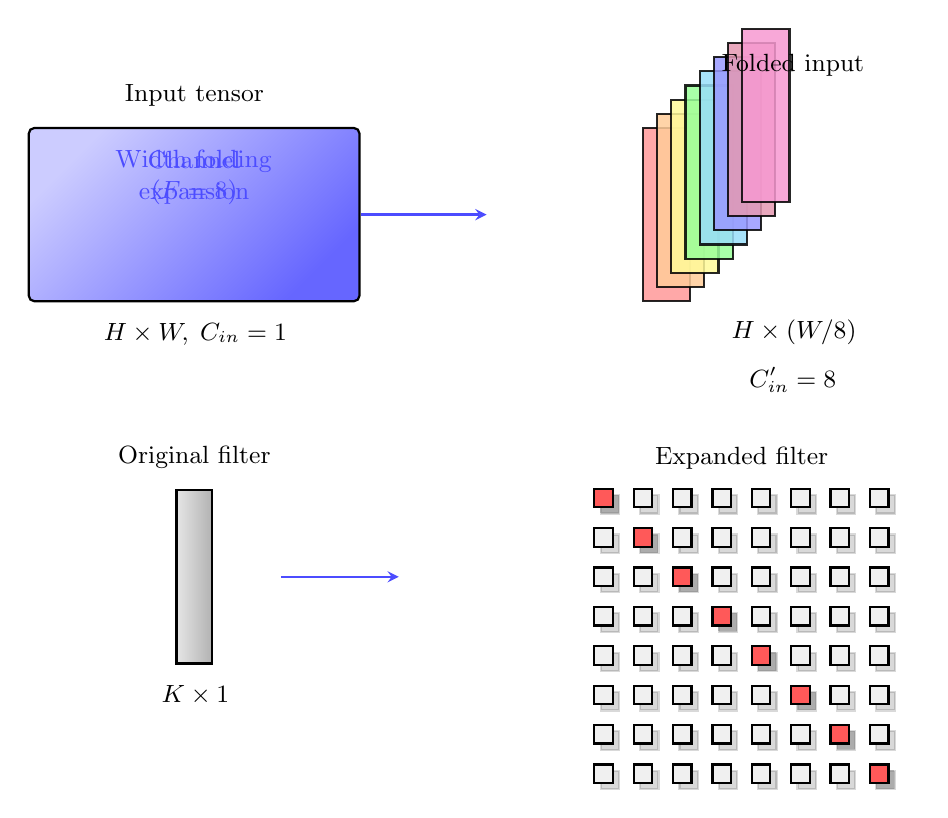
\begin{tikzpicture}[font=\small,>=stealth]

% =========================
% Styles (ALL IN ONE BLOCK)
% =========================
\tikzset{
    tensor/.style={draw, thick, rounded corners=2pt, top color=#1!20, bottom color=#1!60, shading angle=45},
    depth/.style={draw, thick, fill=#1!40, opacity=0.85},
    kernel3d/.style={draw, thick, left color=gray!20, right color=gray!60},
    cell/.style={draw, thick, fill=gray!12},
    diag/.style={draw, thick, fill=red!65, drop shadow},
    arrow/.style={->, thick, color=blue!70}
}

% =========================
% Original Input Tensor (H x W, C=1)
% =========================
\node[tensor=blue, minimum height=2.2cm, minimum width=4.2cm] (orig) at (0,0) {};
\node[above=4pt of orig] {\parbox{2.5cm}{\centering Input tensor}};
\node[below=4pt of orig] {\parbox{2.5cm}{\centering $H \times W,\; C_{in}=1$}};

% =========================
% Width Folding Arrow
% =========================
\draw[arrow] (orig.east) to[out=0,in=180] ++(1.6,0)
    node[midway,above]{\parbox{2.5cm}{\centering Width folding ($F=8$)}};

% =========================
% Folded Input (Channel Depth = 8)
% =========================
\begin{scope}[shift={(6,0)}]
    \foreach \i/\c in {0/red,1/orange,2/yellow,3/green,4/cyan,5/blue,6/purple,7/magenta} {
        \node[depth=\c, minimum height=2.2cm, minimum width=0.6cm] at (\i*0.18,\i*0.18) {};
    }
    \node at (1.6,1.9) {\parbox{3cm}{\centering Folded input}};
    \node at (1.6,-1.5) {\parbox{3cm}{\centering $H \times (W/8)$}};
    \node at (1.6,-2.1) {\parbox{3cm}{\centering $C_{in}' = 8$}};
\end{scope}

% =========================
% Original Filter
% =========================
\begin{scope}[shift={(0,-4.6)}]
    \node[kernel3d, minimum width=0.45cm, minimum height=2.2cm] (filt) at (0,0) {};
    \node[above=4pt of filt] {\parbox{2.5cm}{\centering Original filter}};
    \node[below=4pt of filt] {\parbox{2.5cm}{\centering $K \times 1$}};
\end{scope}

% =========================
% Filter Expansion Arrow
% =========================
\draw[arrow] (1.1,-4.6) to[out=0,in=180] (2.6,-4.6)
    node[midway,above]{\parbox{2.5cm}{\centering Channel expansion}};

% =========================
% Expanded Diagonal Filter (8 x 8)
% =========================
\begin{scope}[shift={(5.2,-3.6)}, yscale=-1]
    % Shadow (3D effect)
    \begin{scope}[opacity=0.15]
        \foreach \i in {0,...,7} {
            \foreach \j in {0,...,7} {
                \node[cell, fill=black] at (\j*0.5+0.08, \i*0.5+0.08) {};
            }
        }
    \end{scope}

    % Main grid
    \foreach \i in {0,...,7} {
        \foreach \j in {0,...,7} {
            \ifnum\j=\i
                \node[cell,diag] at (\j*0.5,\i*0.5) {};
            \else
                \node[cell] at (\j*0.5,\i*0.5) {};
            \fi
        }
    }

    \node at (1.75,-0.5) {\parbox{3cm}{\centering Expanded filter}};
    %\node at (1.75,-1.1) {\parbox{3cm}{\centering Diagonal replication}};
    %\node at (1.75,-1.7) {\parbox{3cm}{\centering $C_{in}' = 8$}};
\end{scope}

\end{tikzpicture}%
}
\caption{
Semantic-preserving CNN reformulation via width folding.
The input width is partitioned into $F=8$ interleaved slices and stacked along the channel dimension, increasing the effective number of input channels without altering spatial height.
The original $K \times 1$ convolution kernel is replicated along the main diagonal of the expanded filter matrix, ensuring independent convolution of each folded slice.
}
\label{fig:full-width-folding}
\end{figure}

%\clearpage       % start on a fresh page
%\onecolumn

\begin{figure}[t]  % t = top of page
\centering
\small  % optional: reduce font to fit vertically
\resizebox{\columnwidth}{!}{%
\begin{minipage}{\columnwidth}
\begin{algorithm}[H]
\caption{Width-Folding Transformation for Convolution}
\label{alg:width-folding}
\begin{algorithmic}[1]
\REQUIRE
Input tensor $X \in \mathbb{R}^{B \times H \times W \times C_{\text{in}}}$, \\
Filter tensor $W_f \in \mathbb{R}^{K_H \times K_W \times C_{\text{in}} \times C_{\text{out}}}$, \\
Bias $b \in \mathbb{R}^{C_{\text{out}}}$, \\
Folding factor $F$

\ENSURE
Transformed tensors $(X_f, W_f', b')$ or fallback

\IF{$W \bmod F \neq 0$}
    \STATE \textbf{return} $(X, W_f, b)$ \COMMENT{Fallback: width not divisible by F}
\ENDIF

\STATE Define $X_f \in \mathbb{R}^{B \times H \times (W/F) \times F}$

\FOR{$b\_idx = 0$ to $B-1$}
    \FOR{$h = 0$ to $H-1$}
        \FOR{$w' = 0$ to $(W/F)-1$}
            \FOR{$f = 0$ to $F-1$}
                \STATE $X_f[b\_idx,h,w',f] \gets X[b\_idx,h,F \cdot w' + f,0]$
            \ENDFOR
        \ENDFOR
    \ENDFOR
\ENDFOR

\STATE Define $W_f' \in \mathbb{R}^{K_H \times K_W \times F \times (F \cdot C_{\text{out}})}$, initialize to zero

\FOR{$f = 0$ to $F-1$}
    \STATE $W_f'[:,:,f,f\cdot C_{\text{out}}:(f+1)\cdot C_{\text{out}}] \gets W_f[:,:,0,:]$
\ENDFOR

\STATE Define $b' \in \mathbb{R}^{F \cdot C_{\text{out}}}$

\FOR{$f = 0$ to $F-1$}
    \STATE $b'[f\cdot C_{\text{out}}:(f+1)\cdot C_{\text{out}}] \gets b$
\ENDFOR

\STATE \textbf{return} $(X_f, W_f', b')$
\end{algorithmic}
\end{algorithm}
\end{minipage}%
}
\end{figure}

\section{Space Folding Transformation}
\label{sec:spacefolding}

For clarity of exposition, the remainder of this paper focuses on
\emph{width folding}, i.e., applying space folding along the width dimension of
convolutional tensors. In a standard convolution, input tensors are structured
as $N \times H \times W \times C$, where $N$ denotes batch size, $H$ height, $W$
width, and $C$ channels. Width folding re-associates the $W$ dimension into the
channel dimension. This choice is made purely for presentation simplicity and
does not restrict the generality of the technique. Space folding applies
equally to the height dimension, or to combinations of spatial dimensions,
whenever the convolution semantics do not mix values across the folded axis.

Given an input tensor
\[
X \in \mathbb{R}^{H \times W \times C_{in}}, \quad C_{in}=1,
\]
and a 1-D convolution kernel
\[
W_f \in \mathbb{R}^{K \times 1},
\]
we fold the width dimension by a factor $F$ such that $W$ is divisible by $F$.
The transformation produces an equivalent convolution with
\[
C_{in}' = F, \quad W' = W / F,
\]
while preserving exact convolution semantics.

\subsection{Input Width Folding}

The width folding operation partitions the width dimension into $F$ interleaved
slices and stacks them along the channel dimension.
Formally, the transformed input tensor
\[
X' \in \mathbb{R}^{H \times (W/F) \times F}
\]
is defined as
\begin{equation}
X'(h, w', f) = X(h, Fw' + f),
\quad
f = 0,\ldots,F-1.
\label{eq:width_fold_def}
\end{equation}

This operation is a pure re-indexing and does not alter the numerical values of
the input tensor.

\subsection{Filter Construction}

Because convolution is performed only along the height dimension, each width
slice is convolved independently.
To preserve this behavior after folding, the original filter is replicated
across the expanded channel dimension without introducing cross-channel mixing.

Let the original filter be
\[
W_f \in \mathbb{R}^{K \times 1}.
\]
We construct a new filter tensor
\[
W_f' \in \mathbb{R}^{K \times F \times F}
\]
as a diagonal replication:
\begin{equation}
W_f'(k, f, f')
=
\begin{cases}
W_f(k), & f = f', \\
0, & f \neq f'.
\end{cases}
\label{eq:filter_construct}
\end{equation}

In implementation terms, this corresponds to allocating a zero-initialized
filter tensor and copying the original filter into the diagonal channel blocks.
Conceptually, each folded width slice receives an identical copy of the
original kernel.

\subsection{Bias Construction}

The original convolution bias
\[
b \in \mathbb{R}
\]
is shared across all folded slices.
Accordingly, the new bias vector is constructed by replication:
\begin{equation}
b'(f) = b,
\quad
f = 0,\ldots,F-1.
\label{eq:bias_construct}
\end{equation}

This ensures that each expanded channel applies the same bias as in the
original formulation.

\subsection{Resulting Convolution}

After width folding and filter construction, the transformed convolution
operates on
\[
X' \in \mathbb{R}^{H \times (W/F) \times F}
\]
using the filter $W_f'$ and bias $b'$.
As shown in Section~\ref{sec:correctness}, this convolution produces outputs
that are exactly equivalent to those of the original network, up to a
bijective re-indexing of the width dimension. The algorithm for computing
width folded convolution is presented in ~\ref{alg:width-folding}.


\section{Space Folding: Mathematical Perspective}
\label{sec:math}

Space folding is a structural transformation of convolutional tensors that trades spatial width for additional channels. Given an input tensor 
$X \in \mathbb{R}^{B \times H \times W \times C_{\text{in}}}$ 
and a folding factor $F$, width folding produces 
$X_f \in \mathbb{R}^{B \times H \times (W/F) \times (C_{\text{in}} \cdot F)}$, via a linear isomorphism
\[
X_f[b,h,w',c'] = X[b,h,F \cdot w' + f, c], \quad c' = f \cdot C_{\text{in}} + c,
\]
preserving all input information. Conceptually, this is equivalent to reindexing the contraction indices in convolution, where the standard contraction
\[
Y[b,h,w,c_{\text{out}}] = \sum_{k_h,k_w,c_{\text{in}}} X[b,h+k_h,w+k_w,c_{\text{in}}]\, W[k_h,k_w,c_{\text{in}},c_{\text{out}}]
\]
becomes, after width folding,
\[
Y_f[b,h,w',c'_{\text{out}}] = \sum_{k_h,k_w,c'_{\text{in}}} X_f[b,h+k_h,w',c'_{\text{in}}]\, W_f'[k_h,k_w,c'_{\text{in}},c'_{\text{out}}].
\]

In linear algebra terms, folding flattens width into channels, allowing the convolution to be represented as a block-diagonal matrix multiplication, where each block corresponds to one slice along the folded width. This structure is naturally interpreted as a Kronecker product: the expanded kernel $W_f'$ can be viewed as the Kronecker product of the original kernel with an identity along the folded width dimension, which aligns well with hardware vectorization and parallelism.

From a category-theoretic viewpoint, tensors are objects in a monoidal category (e.g., $\mathbf{Vect}_\mathbb{R}$) and convolution is a morphism 
$X \otimes W \to Y$. Space folding is a natural isomorphism of the form
\[
B \otimes H \otimes W \otimes C_{\text{in}} \cong B \otimes H \otimes W' \otimes (C_{\text{in}} \otimes F),
\]
reassociating the tensor factors without changing the underlying morphism. Thus, folding is a structure-preserving transformation: the semantics of convolution remain identical, while the indexing structure changes to facilitate computation.

Overall, width folding unifies perspectives from tensor reshaping, contraction, block-diagonal / Kronecker structures, and categorical isomorphisms, providing a concise mathematical framework for this hardware-oriented optimization. The mathematical correctness proof for the transform is provided in Appendinx~\ref{app:correctness}.

\section{Space Folding Transformation as an IR Transformation} 
\label{sec:irtransform}

\subsection{Motivation}

Formulating width-folding as a compiler transformation is feasible and essential because it decouples the mathematical optimization from any particular library or runtime. By representing the input reorganization and kernel replication at the IR level, the compiler can reason about the data layout, tiling, and vectorization systematically. This enables automatic generation of hardware-efficient code that maximizes utilization of compute units such as Tensor Cores, while preserving the semantics of the original convolution. Treating it as a compiler pass ensures portability, composability with other optimizations, and the ability to target multiple backends without manual intervention.


\subsection{Mathematical Formulation}

Let the input tensor be 
$\mathcal{X} \in \mathbb{R}^{B \times H \times W \times C_{\text{in}}}$, 
and the kernel be 
$\mathcal{K} \in \mathbb{R}^{K_H \times K_W \times C_{\text{in}} \times C_{\text{out}}}$, 
producing output 
$\mathcal{Y} \in \mathbb{R}^{B \times H' \times W' \times C_{\text{out}}}$. 

The \emph{width-folding} transformation reshapes the input tensor along the width dimension.
F (folding factor) is chosen to align with Tensor core tile sizes.

\begin{equation}
\mathcal{X}_f \in \mathbb{R}^{B \times H \times \frac{W}{F} \times (C_{\text{in}} \cdot F)}, \quad
F \in \mathbb{Z}^+ 
\end{equation}

The kernel is correspondingly transformed into a diagonal-blocked form:

\begin{equation}
\mathcal{K}_f \in \mathbb{R}^{K_H \times \frac{K_W}{F} \times (C_{\text{in}} \cdot F) \times (C_{\text{out}} \cdot F)}.
\end{equation}

The transformed convolution preserves the original semantics:

\begin{equation}
\mathcal{Y} = \text{Conv}(\mathcal{X}, \mathcal{K}) = \text{Reconstruct}\big(\text{Conv}(\mathcal{X}_f, \mathcal{K}_f)\big),
\end{equation}

where the reconstruction step involves reshaping the folded output back to the original width dimension.

\subsection{Compiler-Level Realization in MLIR}

Space-folding can be potentially implemented as a {\em semantics-preserving IR transformation in MLIR}. The transformation shall be performed over \texttt{linalg.conv\_2d\_nhwc} or \texttt{linalg.matmul} operations, and potentially consist of the following steps:

\begin{enumerate}
    \item \textbf{Tensor Reshape}: Reshape the input and output tensors to introduce a blocked channel dimension corresponding to the folding factor $F$.
    \item \textbf{Affine Reindexing}: Map the original convolution indices to the folded tensor indices, ensuring that all data dependencies are preserved.
    \item \textbf{Kernel Replication}: Replicate the kernel into a diagonal-blocked layout that is consistent with the folded input tensor.
\end{enumerate}

The legality of this transformation is straightforward: the width dimension must be divisible by $F$, and any padding must be applied consistently to preserve output shape. A lightweight cost model can estimate profitability by considering channel size, tensor core tile alignment, and arithmetic intensity.
The transformation is fully composable with other MLIR passes such as tiling, vectorization, and lowering to CUDA or ROCm backends. Space folding thus provides a mathematically sound, hardware-aware optimization that can significantly improve performance of deep learning kernels in production compilers.

\section{Generalization to GEMM via $1 \times 1$ Convolution}
\label{sec:GEMM}


\begin{figure}[h!]
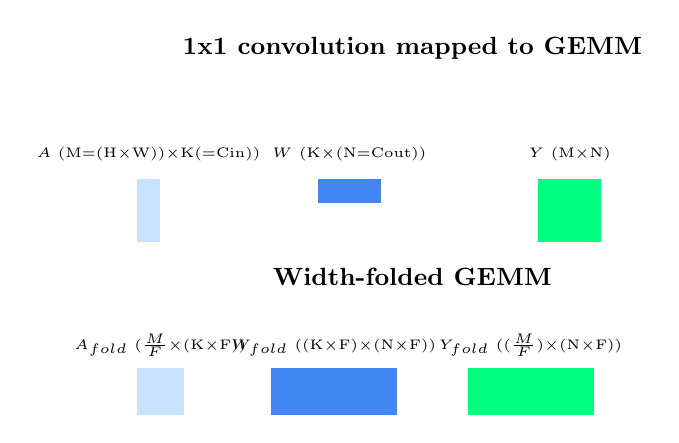
\begin{tikzpicture}[every node/.style={transform shape}]

% ------------------------
% Colors
% ------------------------
\definecolor{colA}{RGB}{198,226,255}
\definecolor{colW}{RGB}{66,134,244}
\definecolor{colY}{RGB}{0,255,128}

% Size of each tiny square
\def\s{0.1} % 0.05cm = very tiny square

% Space between matrices in top row
\def\gap{2.0} % gap in cm
\def\gapb{1.0} % gap in cm

% ------------------------
% TOP ROW: Original GEMM with gaps
% ------------------------
% A: 64x3
\foreach \i in {0,...,7} {
    \foreach \j in {0,...,2} {
        \fill[colA] (\j*\s, -\i*\s) rectangle ++(\s,\s);
    }
}
	\node[above=0.1cm, font=\tiny] at (1.5*\s, 0.1) {$A$ (M=(H$\times$W))$\times$K(=Cin))};

% W: 3x8 (shifted by gap)
\foreach \i in {0,...,2} {
    \foreach \j in {0,...,7} {
        \fill[colW] (3*\s + \gap + \j*\s, -\i*\s) rectangle ++(\s,\s);
    }
}
	\node[above=0.1cm, font=\tiny] at (3*\s + \gap + 4*\s, 0.1) {$W$ (K$\times$(N=Cout))};
\node[above=1cm, font=\small\bfseries] at (3.5,0.5) {1x1 convolution mapped to GEMM};

% Y: 64x8 (shifted by gap after W)
\foreach \i in {0,...,7} {
    \foreach \j in {0,...,7} {
        \fill[colY] (3*\s + \gap + 8*\s + \gap + \j*\s, -\i*\s) rectangle ++(\s,\s);
    }
}
\node[above=0.1cm, font=\tiny] at (3*\s + \gap + 8*\s + \gap + 4*\s, 0.1) {$Y$ (M$\times$N)};

% ------------------------
% BOTTOM ROW: Width-Folded GEMM (fully packed)
% ------------------------
\def\Yshift{-24*\s}

% Colors
\definecolor{colAfold}{RGB}{198,226,255}
\definecolor{colWfold}{RGB}{66,134,244}
\definecolor{colYfold}{RGB}{0,255,128}

% A_fold: 8x24
\foreach \i in {0,...,5} {
    \foreach \j in {0,...,5} {
        \fill[colAfold] (\j*\s, \Yshift-\i*\s) rectangle ++(\s,\s);
    }
}
	\node[above=0.1cm, font=\tiny] at (3*\s, \Yshift+0.02) {$A_{fold}$ ($\frac{M}{F}$$\times$(K$\times$F))};

% W_fold: 24x64
\foreach \i in {0,...,5} {
    \foreach \j in {0,...,15} {
        \fill[colWfold] (7*\s+\j*\s + \gapb, \Yshift-\i*\s) rectangle ++(\s,\s);
    }
}
\node[above=0.1cm, font=\tiny] at (25*\s, \Yshift+0.02) {$W_{fold}$ ((K$\times$F)$\times$(N$\times$F))};

% Y_fold: 8x64
\foreach \i in {0,...,5} {
    \foreach \j in {0,...,15} {
        \fill[colYfold] (22*\s+\j*\s + 2 * \gapb, \Yshift-\i*\s) rectangle ++(\s,\s);
    }
}
\node[above=0.1cm, font=\tiny] at (50*\s, \Yshift+0.02) {$Y_{fold}$ (($\frac{M}{F}$)$\times$(N$\times$F))};
\node[above=1cm, font=\small\bfseries] at (3.5,  \Yshift+0.02) {Width-folded GEMM};

\end{tikzpicture}
\caption{Equivalance between 1x1 convolution and GEMM; followed by width folded GEMM.}
\label{fig:equivalence}
\end{figure}



While width folding is introduced in the context of convolutional operators, the underlying idea extends naturally to general matrix multiplication (GEMM). This follows from the well-known equivalence between GEMM and $1 \times 1$ convolution under appropriate reshaping. We describe this equivalence and show how width folding applies directly to GEMM through this formulation.

\subsection{GEMM as a $1 \times 1$ Convolution}

Consider a matrix multiplication
\[
C = A B,
\]
where $A \in \mathbb{R}^{M \times K}$ and $B \in \mathbb{R}^{K \times N}$.

We reshape matrix $A$ into a tensor
\[
X \in \mathbb{R}^{H \times W \times C_{\text{in}}},
\]
by choosing
\[
H = M, \quad W = 1, \quad C_{\text{in}} = K,
\]
and interpreting each row of $A$ as a spatial position with $K$ channels.

Similarly, matrix $B$ is reshaped into a $1 \times 1$ convolution kernel
\[
W_f \in \mathbb{R}^{1 \times 1 \times C_{\text{in}} \times C_{\text{out}}},
\]
with $C_{\text{out}} = N$.

Applying a $1 \times 1$ convolution produces an output tensor
\[
Y \in \mathbb{R}^{H \times 1 \times C_{\text{out}}},
\]
which is equivalent to the GEMM result $C$ after reshaping.

This construction is algebraically exact and introduces no approximation.

\subsection{Applying Space Folding to GEMM}

In this formulation, the channel dimension corresponds to the reduction dimension $K$ of the matrix multiplication. When $K$ is small or poorly aligned with hardware tile sizes, the resulting computation underutilizes specialized matrix-multiply units.

Space folding can be applied by reindexing an auxiliary spatial dimension and redistributing it into the channel dimension. Concretely, we introduce a synthetic width dimension $W$ and fold it into channels:
\[
X \in \mathbb{R}^{H \times W \times 1}
\;\;\rightarrow\;\;
X' \in \mathbb{R}^{H \times (W/F) \times F}.
\]

The corresponding $1 \times 1$ kernel is replicated into a block-diagonal form, exactly as in the convolutional case. The resulting operator remains a $1 \times 1$ convolution and is therefore equivalent to a GEMM with expanded effective channel dimensionality.

This equivalence shows that width folding is not specific to convolutional layers, but applies more broadly to linear operators expressed as tensor contractions. From a compiler perspective, GEMM and convolution differ only in indexing structure, and both can benefit from operator-level reformulation. This observation further supports expressing width folding as a general compiler transformation rather than a domain-specific optimization.



\section{Potential Optimizations for Sparsity and Quantization}
Efficient exploitation of sparsity is crucial for both memory savings and computational acceleration. The block-diagonal filter structure introduces structured sparsity that can be leveraged in multiple ways. Only the diagonal blocks of the filters contain non-zero values, while off-diagonal blocks are zero. This structured sparsity allows storing just the non-zero blocks in memory as sparse tensors, significantly reducing memory footprint. For large networks, this can lead to substantial savings, especially in embedded or GPU-constrained environments. Several modern deep learning frameworks and custom CUDA kernels can exploit this by performing sparse matrix multiplications, reducing the number of operations and increasing throughput. Popular deep learning frameworks such as PyTorch and TensorFlow provide built-in support for grouped convolutions. By mapping each diagonal block to a group, the block-diagonal convolution can be implemented efficiently without modifying the core framework. 
    
Structured sparsity pairs naturally with mixed-precision quantization (FP16/INT8). By representing both weights and activations in lower precision, memory bandwidth is reduced, and Tensor Cores can achieve higher throughput. Combining quantization with block-diagonal sparsity ensures that only essential computations are performed at high speed, improving overall efficiency while maintaining model accuracy.


%\twocolumn

\section{Results}
\label{sec:evaluation}

We implemented the width-folding transformation in TensorFlow and TensorRT, validating it against functionally equivalent convolutions. Since TensorRT does not provide a programmable transformation IR, space folding is lowered \emph{by hand} by explicitly constructing an equivalent TensorRT graph. The lowering materializes the folded layout via reshaping spatial dimensions and replicating convolution filters to preserve receptive-field semantics. All semantic correctness is established at the IR level prior to lowering; TensorRT is used only for kernel selection, layout specialization, and execution. At this time, we did not explore MLIR-based lowering to TensorRT; investigating a principled MLIR lowering pipeline is left as future work. A representative TensorFlow implementation is provided in Appendix~\ref{app:reference}.

We executed our experiments on a \textbf{NVIDIA RTX PRO 5000 Blackwell} GPU with \textbf{CUDA 13.1} and \textbf{TensorRT 1.3.0.35}. Folding fator (F) of 8 and FP16 precision was used in all experiments. Results were already summarized in the Figure~\ref{fig:sensitivity}. We highlight few additional results here, using input feature maps of size $H=64$ and $W=1024$. Figure~\ref{fig:perf} shows the execution time of the reference convolution versus the proposed width-folded implementation. For \mbox{1$\times$1} filters, width folding reduces execution time from \textbf{0.0114 ms} to \textbf{0.0043 ms}, achieving a \textbf{2.65$\times$ speedup}. For \mbox{3$\times$1} filters, execution time drops from \textbf{0.0120 ms} to \textbf{0.0051 ms}, a \textbf{2.35$\times$ speedup}. We obtain similar speedup for filter of size \mbox{5$\times$1}. We repeated the experiments with stride=8 and observed similar speeups too. 

Using $tensort\_rtx$ (an measurement tool provided as part of TensorRT), we observed that the reference engine allocates 393,216 bytes of workspace during execution, whereas the width-folded engine requires zero scratch memory. This confirms that the memory reduction arises from space folding optimization. We hypothesize that the reference formulation introduces explicit padding along the width dimension, which forces TensorRT to select tactics that require temporary workspace. In contrast, width folding removes the padded dimension from the problem geometry, enabling a direct convolution kernel that requires no scratch memory during execution.  Space saving is important as that will enable to use models with large channel count. All these results demonstrate that width folding significantly reduces computation and memory overhead while maintaining the original convolution semantics, with consistent performance gains across filter sizes.  

TensorRT is already highly optimized; achieving $\approx3\times$ performance improvement indicates a fundamentally new algorithmic approach, improved hardware utilization, and domain-specific optimization beyond generic kernels.  The primary source of performance improvement is the avoidance of tensor reformatting overhead. Vanilla TensorRT often inserts implicit layout transformations before and after convolution to satisfy hardware alignment constraints,  which adds memory traffic and computational cost. TensorRT supports several input/output formats, including \texttt{kHWC8}, where the last dimension (channels) is padded to a multiple of 8. The 'k' prefix indicates a blocked format suitable for Tensor Cores, and 'HWC8' signifies that 8 channels are stored contiguously. Another format is \texttt{CHW4}. Space folding directly produces tensors in this aligned format without additional runtime reordering, eliminating memory-bound operations and reducing latency.


\begin{figure}[t]
\centering
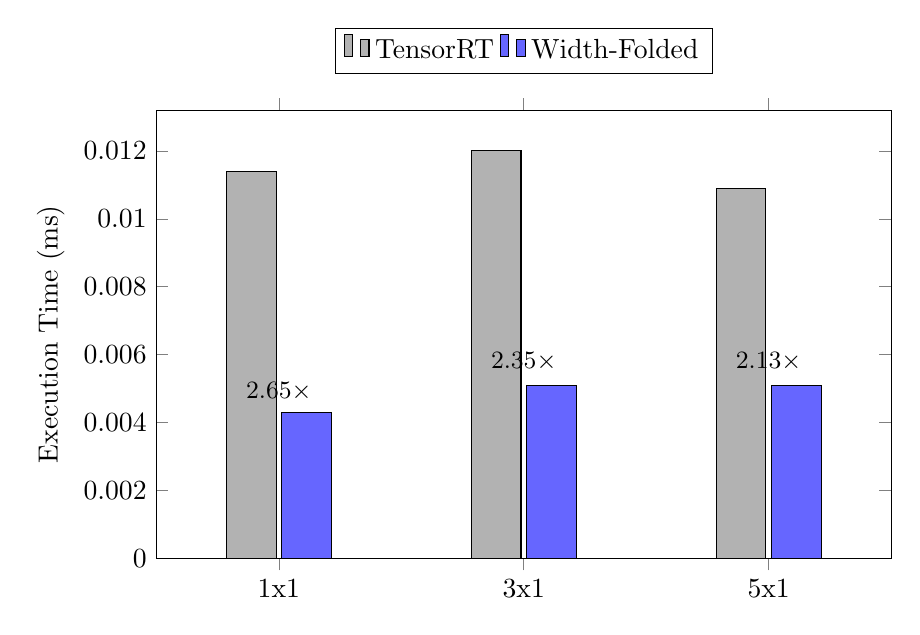
\begin{tikzpicture}
\begin{axis}[
    ybar,
    bar width=18pt,
    width=0.9\columnwidth,
    height=0.6\columnwidth,
    ymin=0,
    ylabel={Execution Time (ms)},
    symbolic x coords={1x1,3x1,5x1},
    xtick=data,
    legend style={at={(0.5,1.08)},anchor=south,legend columns=2},
    scaled y ticks=false,
    yticklabel style={/pgf/number format/fixed,/pgf/number format/precision=4},
    enlarge x limits=0.25
]

% Reference bars (TensorRT)
\addplot[
    bar shift=-10pt,
    fill=gray!60,
    draw=black
] coordinates {
    (1x1,0.0114)
    (3x1,0.0120)
    (5x1,0.0109)
};

% Width-folded bars (blue)
\addplot[
    bar shift=10pt,
    fill=blue!60,
    draw=black
] coordinates {
    (1x1,0.0043)
    (3x1,0.0051)
    (5x1,0.0051)
};

% Speedup annotations
\node at (axis cs:1x1,0.0049) {\small 2.65$\times$};
\node at (axis cs:3x1,0.0058) {\small 2.35$\times$};
\node at (axis cs:5x1,0.0058) {\small 2.13$\times$};

\legend{TensorRT,Width-Folded}

\end{axis}
\end{tikzpicture}
\caption{Execution time comparison between standard TensorRT and width-folded convolutions, Cin = Cout = Stride=1.
Speedups over TensorRT are annotated above the blue bars. Space folding avoids pre/post convolution reformatting, enabling higher Tensor Core utilization.}
\label{fig:perf}
\end{figure}

\begin{figure}[t]
\centering
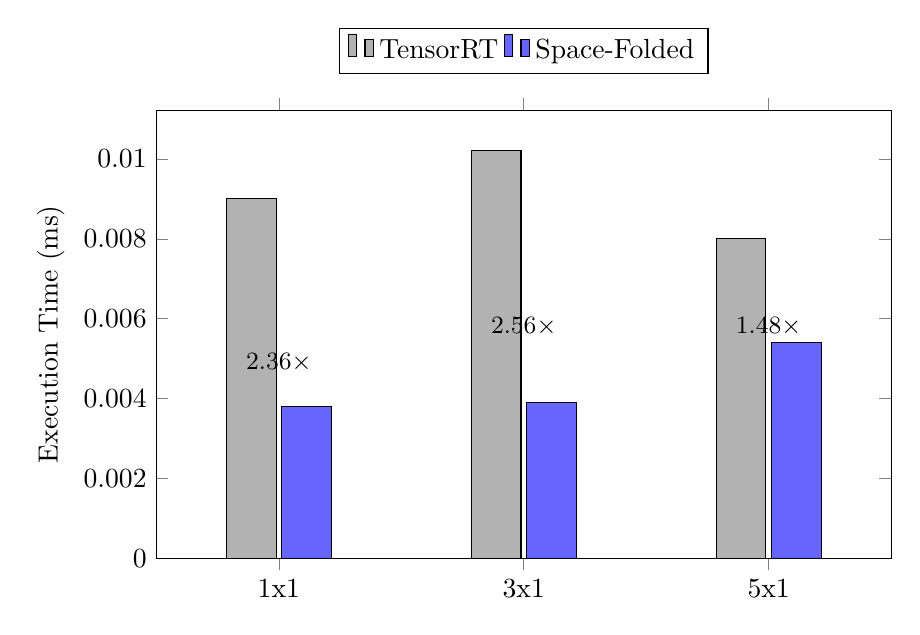
\begin{tikzpicture}
\begin{axis}[
    ybar,
    bar width=18pt,
    width=0.9\columnwidth,
    height=0.6\columnwidth,
    ymin=0,
    ylabel={Execution Time (ms)},
    symbolic x coords={1x1,3x1,5x1},
    xtick=data,
    legend style={at={(0.5,1.08)},anchor=south,legend columns=2},
    scaled y ticks=false,
    yticklabel style={/pgf/number format/fixed,/pgf/number format/precision=4},
    enlarge x limits=0.25
]

% Reference bars (TensorRT)
\addplot[
    bar shift=-10pt,
    fill=gray!60,
    draw=black
] coordinates {
    (1x1,0.0090)
    (3x1,0.0102)
    (5x1,0.0080)
};

% Width-folded bars (blue)
\addplot[
    bar shift=10pt,
    fill=blue!60,
    draw=black
] coordinates {
    (1x1,0.0038)
    (3x1,0.0039)
    (5x1,0.0054)
};

% Speedup annotations
\node at (axis cs:1x1,0.0049) {\small 2.36$\times$};
\node at (axis cs:3x1,0.0058) {\small 2.56$\times$};
\node at (axis cs:5x1,0.0058) {\small 1.48$\times$};

\legend{TensorRT,Space-Folded}

\end{axis}
\end{tikzpicture}
\caption{Execution time comparison between standard TensorRT and width-folded convolutions with Cin=Cout=1 and stride=8.
Speedups over TensorRT are annotated above the blue bars. Space folding avoids pre/post convolution reformatting, enabling higher Tensor Core utilization.}
\label{fig:perf-stride8}
\end{figure}



In addition to synthetic tests, industrial experiments conducted on a wide range of real-world CNNs (as reported in~\cite{roche_pct}) consistently demonstrate a minimum of 3$\times$ speedups on NVIDIA A100 GPUs, for first layers of CNN networks.  
%\texttt{cuDNN} ~\cite{chetlur2014cudnn}, another popular deep learning framework, exposes FP16 convolution at the API level. However, convolutions with very small input channel counts—most notably $C_{\text{in}} = 1$—are not allowed by default due to reason that tensor Cores require matrix dimensions that are multiples of 8. For such cases, the responsibility is pushed to the user rather than the library and users must explicitly pad the channel dimension with zeros or use FP32 variant. Zero padding increases memory traffic and performs wasted computation on artificial data, while falling back to FP32 introduces FP16--FP32--FP16 conversion overhead and executes on CUDA cores (not Tensor cores). In both cases, Tensor Cores remain underutilized, despite their theoretical ability to provide up to an $8\times$ throughput improvement for FP16 operations.

%The above facts reflect the design philosophy of TensorRT and cuDNN as a general-purpose kernel library rather than a system that invents new mathematical formulations. They faithfully implement the operation given; they do not reinterpret tensor dimensions or apply semantics-changing transformations to satisfy hardware alignment requirements. In contrast, our approach introduces a semantics-preserving mathematical transformation that increases the effective channel dimension without zero padding or precision up/down-conversion. This reparameterization makes the convolution natively compatible with FP16 Tensor Core kernels, enabling high utilization and substantially higher performance than existing cuDNN or TensorRT implementations for low-channel-count convolutions.


\begin{figure}[t]
\centering
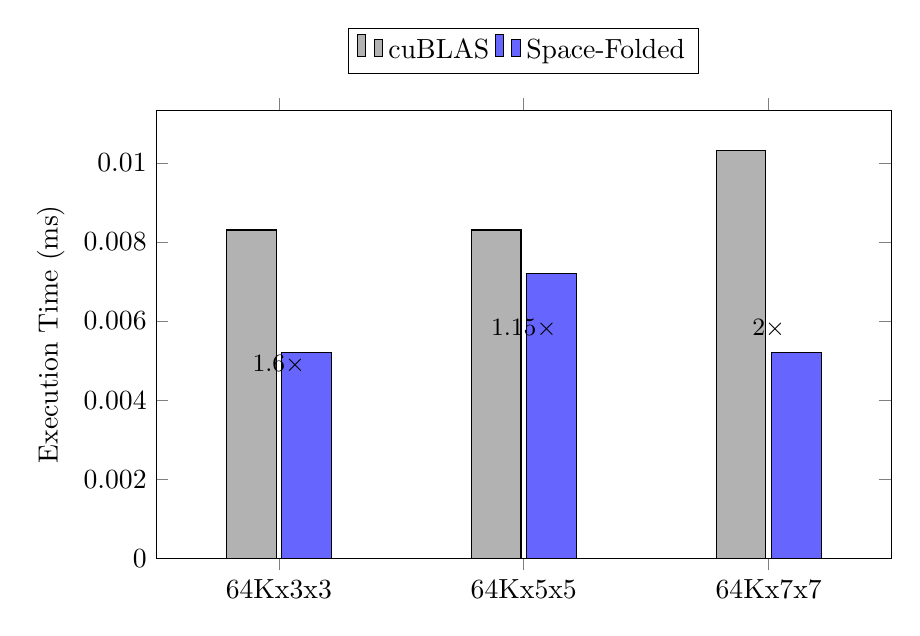
\begin{tikzpicture}
\begin{axis}[
    ybar,
    bar width=18pt,
    width=0.9\columnwidth,
    height=0.6\columnwidth,
    ymin=0,
    ylabel={Execution Time (ms)},
    symbolic x coords={64Kx3x3,64Kx5x5,64Kx7x7},
    xtick=data,
    legend style={at={(0.5,1.08)},anchor=south,legend columns=2},
    scaled y ticks=false,
    yticklabel style={/pgf/number format/fixed,/pgf/number format/precision=4},
    enlarge x limits=0.25
]

% Reference bars (TensorRT)
\addplot[
    bar shift=-10pt,
    fill=gray!60,
    draw=black
] coordinates {
    (64Kx3x3,0.0083)
    (64Kx5x5,0.0083)
    (64Kx7x7,0.0103)
};

% Width-folded bars (blue)
\addplot[
    bar shift=10pt,
    fill=blue!60,
    draw=black
] coordinates {
    (64Kx3x3,0.0052)
    (64Kx5x5,0.0072)
    (64Kx7x7,0.0052)
};

% Speedup annotations
\node at (axis cs:64Kx3x3,0.0049) {\small 1.6$\times$};
\node at (axis cs:64Kx5x5,0.0058) {\small 1.15$\times$};
\node at (axis cs:64Kx7x7,0.0058) {\small 2$\times$};

\legend{cuBLAS,Space-Folded}

\end{axis}
\end{tikzpicture}
\caption{Execution time comparison between 1x1 convolution and equivalent GEMM. (M$\times$N$\times$K).
Speedups are annotated above the blue bars. Space folding provides 2$\times$ speedup for Cin=Cout=7.}
\label{fig:gemm-perf}
\end{figure}

The proposed method applies to any convolutional layer, not just the first layer. The method can also be extended to linear layers (i.e., GEMM) by reformulating as $1\times1$ convolutions as noted in Section~\ref{sec:GEMM}. This extension implies that the transformation could accelerate GEMM operations in cuBLAS (especially, those involving {\em tall skinny matrices}). We executed the space folded convolution and the equivalent GEMM using cuBLAS for various Cin and Cout (chosen to be some odd number). The results are summarized in Figure ~\ref{fig:gemm-perf}. A maximum of $2\times$ speedup over cuBLAS was observed for Cin=Cout=7.



\section{Related Work}
\label{sec:related}

Optimizing CNNs for hardware accelerators has been an active area of research. Our approach draws inspiration from several existing techniques, combining channel expansion and block-diagonal sparsity to fully exploit hardware throughput. 

\subsection{Relation to Other CNN Variants}

Our block-diagonal width-folding transformation is related to grouped~\cite{krizhevsky2012imagenet} and depthwise~\cite{howard2017mobilenets} convolutions in that it introduces structured partitioning and sparsity, but it differs by preserving the original filter values and multi-channel interactions while replicating them solely to satisfy Tensor Core alignment constraints. Unlike space-to-depth transformation~\cite{space2depth}, which alter convolution semantics, or $1\times1$ convolutions that expand representational capacity, our approach maintains exact input--output equivalence and introduces no additional learnable parameters. While conceptually related to low-rank filter approximations~\cite{jaderberg2014speeding} and kernel tiling optimizations~\cite{chetlur2014cudnn}, our method focuses on semantic-preserving operator reformulation rather than approximation, enabling full utilization of modern tensor hardware without modifying the underlying model.

\subsection{Difference from Channel Zero-Padding}

A simple approach to align channels for hardware is \emph{zero-padding}: if a layer has 1 input channel and the hardware prefers multiples of 8, 7 zero channels are added. While this aligns the total channels, these extra channels carry no information, wasting compute on irrelevant data. In contrast, \emph{width-folding} avoids adding input channels, expanding only the (small) weight tensor. It creates \emph{block-diagonal filters}, introducing structured sparsity that frameworks can exploit for efficient computation. Moreover, this pattern naturally generalizes to higher-dimensional and grouped convolutions.


\subsection{Contrast with Traditional Compiler Transformations}

Space (width) folding differs fundamentally from traditional compiler optimizations in deep learning systems. Whereas standard compiler techniques—such as fusion, tiling, layout reordering, vectorization, and kernel selection—optimize *how* a fixed mathematical operator is executed, width folding rewrites the operator itself by re-indexing tensor dimensions and restructuring filters while preserving exact input–output semantics. This explicit, semantics-preserving reformulation enforces hardware alignment constraints directly at the model level, without padding or special-case kernels, making it analyzable and provably correct. Applied post-training but pre-compilation, width folding complements existing compiler optimizations by expanding the space of hardware-friendly operator formulations that downstream compilers can further optimize.

\section{Conclusion}
\label{sec:discussion}
We presented a transformation for CNN filters that aligns input and output channels with NVIDIA Tensor Core requirements. The method maintains the original filter structure, generalizes to n-D convolutions, and exploits sparsity for memory and computational efficiency. This approach bridges hardware-aware optimizations with traditional CNN design principles, providing a practical and scalable solution for high-performance deep learning deployments.

\subsection{Future Work}

Several promising research directions follow naturally. Some are listed below.

\begin{enumerate}
    \item Explore broader \emph{structure-preserving transformations}, including spatial--channel folding, hierarchical blocking, mixed-radix reshaping, sparsity-aware folding, and dilation rewriting. Investigate the mathematical feasibility of the inverse (channel-to-space) transformations.
    
    \item Adapt transformations to diverse hardware, including AMD GPUs and general-purpose CPUs, taking into account wavefront sizes, memory coalescing, matrix instruction formats, and SIMD/block alignment requirements~\cite{onednn2025}.
    
    \item Extend techniques to additional operators commonly used in modern architectures, such as grouped and depthwise separable convolutions, attention mechanisms~\cite{attention,flash3}, and recurrent layers~\cite{lstm}.
    
    \item Support low-precision and alternative data formats, including FP8, FP4, and layouts such as kCHW4 or kCHW16, in TensorRT and oneDNN. Explore applying these transformations during training to achieve speedups and improved tensor core utilization.
    
    \item Integrate transformations into compiler frameworks like MLIR~\cite{mlir}.
\end{enumerate}

%More broadly, we introduce \emph{semantic tuning} as a post-training optimization paradigm in which the mathematical formulation of a neural network is rewritten to better match hardware execution constraints while preserving the exact input–output semantics of the original model. This shifts the compiler optimizations from hardware-specific kernel optimization toward \emph{semantically equivalent operator transformations}, achieving performance portability.

\FloatBarrier
\bibliography{cnn_paper_pldi}
\bibliographystyle{icml2026}

\newpage
\appendix
\onecolumn
% -----------------------------
% In your section where you want the figure
% -----------------------------
\section{Correctness of Space Folding Transformation}
\label{app:correctness}

We consider a 1-D convolution performed exclusively along the height
dimension \(H\).
The width dimension \(W\) does not participate in the convolution and is
treated as an independent indexing dimension.

Let the input tensor be
\[
X \in \mathbb{R}^{H \times W \times C_{in}}, \quad C_{in} = 1,
\]
and let the convolution filter be
\[
W_f \in \mathbb{R}^{K \times 1},
\]
with bias \(b \in \mathbb{R}\).
Batch and output channel indices are omitted for clarity.

The original convolution output is given by
\begin{equation}
Y(h, w)
=
\sum_{k=0}^{K-1}
W_f(k)\, X(h+k, w) + b,
\label{eq:orig_conv_H}
\end{equation}
where convolution is performed only along the height dimension.

\paragraph{Space Folding Transformation.}
Let \(F\) be the folding factor and assume \(W\) is divisible by \(F\).
We define a transformed input tensor
\[
X' \in \mathbb{R}^{H \times (W/F) \times F}
\]
by re-indexing the width dimension as
\begin{equation}
X'(h, w', f)
=
X(h, Fw' + f),
\quad
f = 0,\ldots,F-1.
\label{eq:width_fold}
\end{equation}
This operation folds the width dimension into the channel dimension
without modifying spatial data along \(H\).

\paragraph{Filter Expansion.}
Since the convolution is independent across width indices, the filter
must be replicated for each folded slice.
We define an expanded filter
\[
W_f' \in \mathbb{R}^{K \times F \times F}
\]
as a diagonal replication:
\begin{equation}
W_f'(k, f, f')
=
\begin{cases}
W_f(k), & f = f', \\
0, & f \neq f'.
\end{cases}
\label{eq:diag_filter_H}
\end{equation}
The bias is similarly replicated as \(b'(f) = b\).

\paragraph{Transformed Convolution.}
The output of the transformed convolution is
\begin{equation}
Y'(h, w', f)
=
\sum_{k=0}^{K-1}
\sum_{f'=0}^{F-1}
W_f'(k,f,f')\, X'(h+k, w', f')
+ b'(f).
\label{eq:new_conv_H}
\end{equation}

Substituting Eq.~\eqref{eq:diag_filter_H} into
Eq.~\eqref{eq:new_conv_H} removes the channel summation:
\begin{equation}
Y'(h, w', f)
=
\sum_{k=0}^{K-1}
W_f(k)\, X'(h+k, w', f) + b.
\label{eq:new_conv_simplified_H}
\end{equation}

Using the folded input definition from
Eq.~\eqref{eq:width_fold}, we obtain
\[
Y'(h, w', f)
=
\sum_{k=0}^{K-1}
W_f(k)\, X(h+k, Fw' + f) + b.
\]

Let \(w = Fw' + f\).
Then
\[
Y'(h, w', f) = Y(h, w),
\]
where \(Y(h,w)\) is the output of the original convolution defined in
Eq.~\eqref{eq:orig_conv_H}.

\paragraph{Conclusion.}
The width folding transformation constitutes a bijective re-indexing of
the width dimension combined with diagonal filter replication.
Since the convolution is performed solely along the height dimension,
the transformation preserves the exact numerical output of the original
network.
Therefore, width folding with channel expansion is
\emph{semantics preserving}.
\hfill\(\square\)

Our method generalizes to N-D convolutions by folding dimensions that are not involved in the convolution operation into the channel dimension. This reparameterization preserves exact convolution semantics via block-diagonal kernels and does not rely on kernel separability or approximation.
%\vspace{2mm} % small spacing between figure and code

\section{Example Code using Tensorflow CNN (Channels-Last)}
\label{app:reference}
This Tensorflow implementation demonstrates a 2-D block-diagonal filter transformation where the input is in channels-last format ($[B, H, W, C_in]$), the W dimension is folded, and the convolution is compatible with NVIDIA Tensor Cores.


\lstset{
    language=Python,
    basicstyle=\ttfamily\small,
    keywordstyle=\color{blue},
    commentstyle=\color{green!60!black},
    stringstyle=\color{orange},
    numbers=left,
    numberstyle=\tiny\color{gray},
    stepnumber=1,
    numbersep=5pt,
    showspaces=false,
    showstringspaces=false,
    breaklines=true,
    frame=single,
    caption={Width-folding CNN transformation in TensorFlow (channels-last).},
    label={lst:width_folding}
}

\begin{lstlisting}
import tensorflow as tf
import numpy as np

# -----------------------------
# Parameters
# -----------------------------
B, H, W = 1, 32, 64     # batch, height, width
K = 5                  # kernel size along H
F = 8                  # width folding factor
Cout = 1               # output channels

assert W % F == 0

# -----------------------------
# Input tensor (NHWC)
# -----------------------------
x = tf.random.normal((B, H, W, 1))

# -----------------------------
# Original filter + bias
# Conv along H only -> kernel (K,1)
# -----------------------------
filterVal = tf.random.normal((K, 1, 1, Cout))
biasVal = tf.random.normal((Cout,))

# -----------------------------
# Original convolution
# -----------------------------
y_orig = tf.nn.conv2d(
    x,
    filterVal,
    strides=[1, 1, 1, 1],
    padding="VALID",
    data_format="NHWC"
)
y_orig = tf.nn.bias_add(y_orig, biasVal)

# -----------------------------
# Width folding: W -> W/F, Cin -> F
# -----------------------------
# (B, H, W, 1) -> (B, H, W/F, F)
x_folded = tf.reshape(x, (B, H, W // F, F))

# -----------------------------
# Build diagonal filter
# (K,1,1,Cout) -> (K,1,F,F*Cout)
# -----------------------------
filterValNew = np.zeros((K, 1, F, F * Cout), dtype=np.float32)

for f in range(F):
    filterValNew[:, :, f, f*Cout:(f+1)*Cout] = np.squeeze(filterVal.numpy(),axis=-1)

filterValNew = tf.constant(filterValNew)

# -----------------------------
# Bias replication
# -----------------------------
biasValNew = tf.tile(biasVal, [F])

# -----------------------------
# Folded convolution
# -----------------------------
y_folded = tf.nn.conv2d(
    x_folded,
    filterValNew,
    strides=[1, 1, 1, 1],   # stride only along H
    padding="VALID",
    data_format="NHWC"
)
y_folded = tf.nn.bias_add(y_folded, biasValNew)

# -----------------------------
# Reconstruct original layout
# (B, H', W/F, F) -> (B, H', W)
# -----------------------------
y_reconstructed = tf.reshape(
    y_folded,
    (B, y_folded.shape[1], W)
)

# -----------------------------
# Verification
# -----------------------------
max_error = tf.reduce_max(tf.abs(np.squeeze(y_orig, axis=-1) - y_reconstructed))
print("Max absolute error:", max_error.numpy())

# Assert correctness
tf.debugging.assert_near(np.squeeze(y_orig, axis=-1), y_reconstructed, atol=1e-5)
print("Width folding transformation is numerically correct")
\end{lstlisting}

\end{document}
